%--------------------------------------------------
%	Chapter 5. GNN Pattern Recognition Algorithm
%--------------------------------------------------

\chapter{Graph Neural Network Pattern Recognition Algorithm}\label{chapter-5}

Once compatible hit-pairs from a particle collision event have been established, they can be used to build a graph network. This chapter presents a novel pattern recognition algorithm utilising GNN architectures to prune connections in such a network, in order to reconstruct tracks in a silicon based Pixel detector. The application is focused on the Pixel detector, with the aim that the approach will serve as a sophisticated track seeding technique for Pixel hits and form preliminary track candidates. These seeds can be extended into the Strips using standard track following. Such an approach could be efficient for saving computational resources if the GNN does not produce large proportions of fake tracks. The ultimate aim of this work is to develop a realistic algorithm for fast track reconstruction that can be deployed in future high-luminosity phases of particle detector experiments. This research was presented at the 2022 Connecting the Dots (CTD) conference at the University of Princeton USA and is currently under review for publication in the Springer Journal: Computing for Software and Big Science \cite{Lad_2023_gnn}. Sections \ref{gnn-algorithm-overview} to \ref{gnn-track-extration} presents an overview and detailed breakdown of each stage of the algorithm. Section \ref{gnn-application-toy-model} illustrates a simple application on a toy model.



\section{Algorithm Overview}
\label{gnn-algorithm-overview}
The GNN based pattern recognition algorithm is considered an iterative mixture reduction task, which allows the deactivation of incompatible connections (GNN edges termed as outliers) in order to improve track parameter estimates and iteratively extract track candidates. 

Individual hits or clusters of hits are modelled as graph nodes and track segments are modelled as graph edges. Once the graph network is constructed, each edge is modelled as a Gaussian state in order to approximate the local track state probability density. Therefore, each node is initialised with a Gaussian mixture of track states, local to its neighbourhood of connections.

After initialisation, the network evolves iteratively, where an iteration is made up of three main stages illustrated in Figure \ref{fig:flowchart}. The first stage comprises of Gaussian Mixture Reduction (GMR). This involves a traditional ML approach, whereby compatible Gaussian states are grouped together using clustering techniques and outlier states can be identified. This stage is followed by information aggregation by leveraging message passing between nodes in a given neighbourhood. The compatibility of neighbouring states can be assessed via extrapolation, in order to improve local track parameters using neighbourhood information. The third stage involves updating the network state at each node, as certain connections are deactivated. A graph splitting algorithm is also applied directly after the first two stages to identify good track candidates, and if discovered they are extracted. 

Unlike traditional methodologies whereby Multi-Layered Perceptrons (MLPs) are employed for deep learning strategies, the proposed GNN leverages simplified KFs embedded in the network and are used for two main purposes. Firstly, the KF is used as a mechanism for information propagation, in order to iteratively improve the precision of track parameters. The KF is also used in extraction of track candidates compatible with particle motion model. This allows the model to efficiently exploit a prior knowledge about charged particle dynamics as the network evolves.

The excitation and inhibition rules of individual edge connections are designed to facilitate the “simple-to-complex” approach for “hits-to-tracks” association, such that the network starts with low hit density regions of an event and gradually progresses towards more complex areas. As the network evolves, the uncertainty in local track orientation decreases until there are no more track candidates that fulfil the criteria for a good track. This is the end state of the network where isolated nodes, track fragments and unresolved ambiguities will remain.

\begin{figure}[htbp]
    \centering
    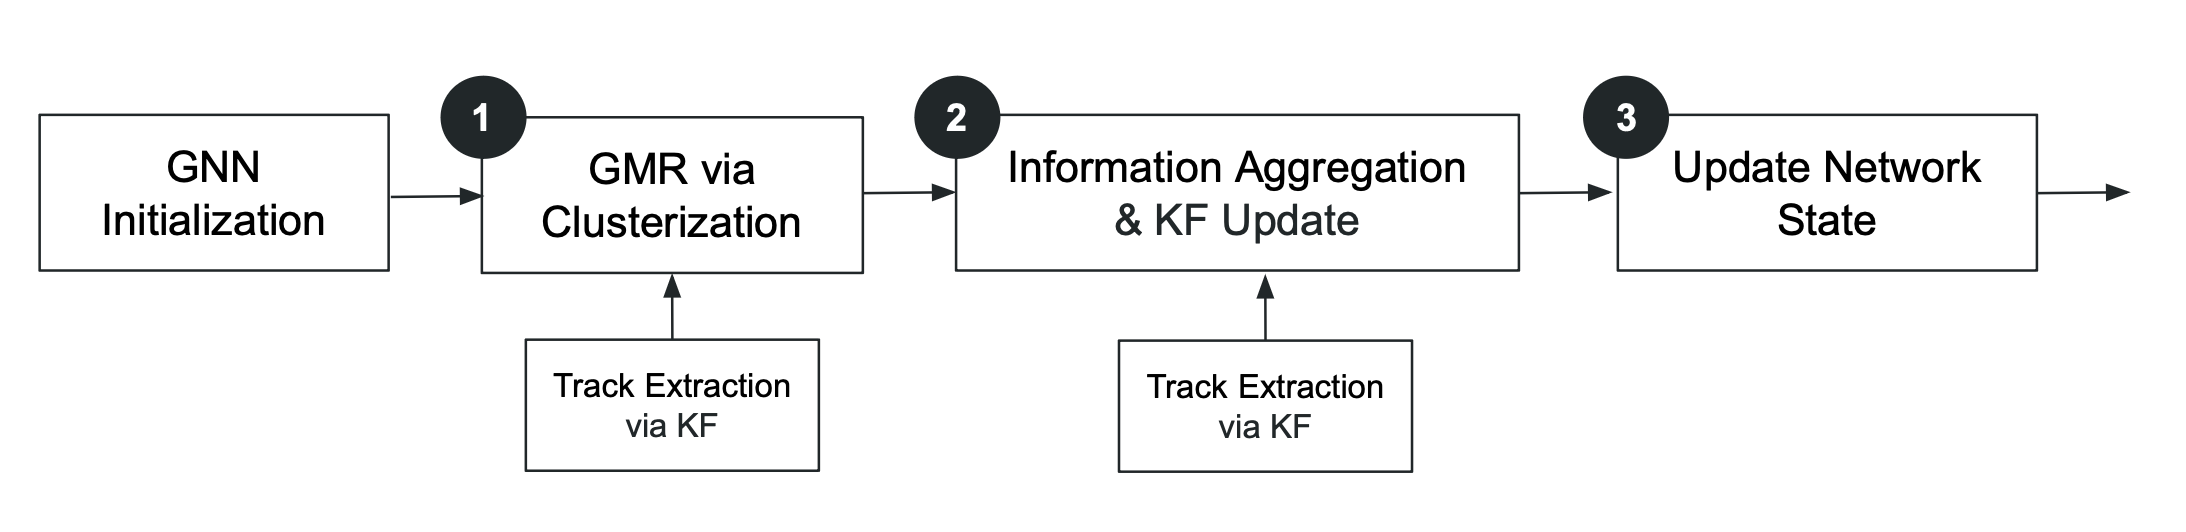
\includegraphics[width=0.98\textwidth]{images/5-gnn-algorithm/gnn-workflow.png}
    \caption{Flow chart illustrating all stages making up an iteration of the GNN-based algorithm. After each stage, a Kalman filter (KF) is applied in order to iteratively extract candidates. After stage three, a further Gaussian Mixture Reduction (GMR) stage would be applied repeating the iterations.}
    \label{fig:flowchart}%
\end{figure}



\section{Graph Network Initialization}
\label{gnn-network-initialization}

The graph network is constructed using the Python library \textit{NetworkX} \cite{SciPyProceedings_11}. Hits from a particle event are represented as nodes and predicted hit-pairs as edge connections. See chapter \ref{chapter-4} for further details on the hit-pair predictor used to form edge connections. Following this, a common computer vision technique, known as Connected Component Analysis (CCA), is applied using a built-in function\cite{networkx}. CCA detects connected regions in data structures and allows the network to be split into smaller, more manageable graphs referred to as \textit{subgraphs}. 

Each pairwise connection between node $i$ and neighbour node $j$ forms a Gaussian state, $X_{ij}$, representing the local track parameter estimate. Each edge has an associated prior probability $p_{ij}$ and edge weight $w_{ij}$. The prior probability of node $i$ and neighbour node $j$ belonging to the same track is determined, assuming a track can produce at most one hit per layer of the detector. $w_{ij}$ is a mixture weight for the compatibility of the Gaussian state transmitted from node $i$ to neighbour node $j$, representing the strength of the connection. $w_{ij}$ are initialised as uniform dependent on the number of neighbours local to a node and are updated based on how the network evolves. $w_{ij}$ are not to be confused with the traditional weights associated to features within neural networks.

For a given node $i$ and neighbour nodes $j$, a Gaussian mixture $g_i(X)$ is formed from weighted components, $\phi_{ij}$, which describe the local neighbourhood and is given by Eq \eqref{eqn:gaussian-mixture},

\begin{equation}
g_i(X) = \sum_{j} w_{ij}\phi_{ij}(X, X_{ij}, C_{ij})
\label{eqn:gaussian-mixture}
\end{equation}

where $C_{ij}$ are the track state covariances. All edges act as bidirectional conduits, such that message passing can occur in both directions. All edges are initialised as \textit{active}, allowing the propagation of state information, whereas \textit{deactive} edges are defined to not allow state information to be propagated. 

%Figure \ref{fig:network-initial} illustrates a node and its neighbourhood.

% \begin{figure}[htbp]%
%     \centering
%     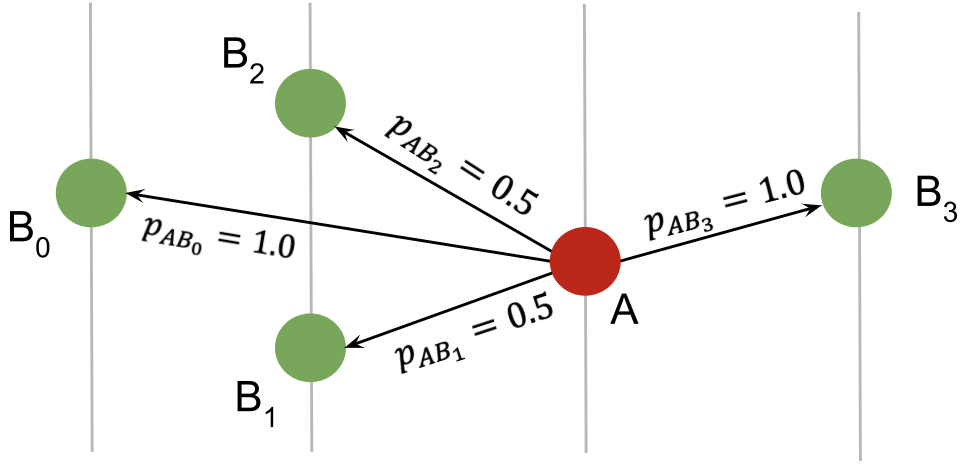
\includegraphics[width=8.8cm]{images/5-gnn-algorithm/network-initialisation.png}%
%     \caption{Prior probabilities associated to network edges of node A's local neighbourhood. Neighbours $B_j$ are located on separate detector layers shown by vertical lines. The unidirectional edges indicate the direction of propagation of state information and priors. These entities will differ from nodes $B_j$ distributing messages to their corresponding neighbourhoods.}%
%     \label{fig:network-initial}%
%\end{figure}




\section{Gaussian Mixture Reduction}
For nodes with a high multiplicity of edge connections, the number of track states can quickly rise. To make inferences within a reasonable amount of processing time, GMR is used to prevent the number of components from exploding. One computationally efficient algorithm for GMR is a clustering. A high order Gaussian mixture is approximated by one with lower order, using the traditional k-means clustering \cite{kmeans}. At each node, similar track states are grouped together forming a reduced mixture and their corresponding edges remain active, as illustrated in Figure \ref{fig:GMR-example}. For a given node $i$, the merged state estimate $X^{M}$ and merged state covariance $C^{M}$ is formed using the clustered states and the inverse-variance weighting \cite{inverse-variance-weighting} given by Eqs \eqref{eqn:inverse-variance-weighting}, where $G_{ij}$ = $C_{ij}^{-1}$. Outlier states are identified and their edges are deactivated.

\begin{equation}
    X^{M} = C^{M} \sum_{j} G_{ij} X_{ij},  \quad  C^{M} = \left( \sum_{j} G_{ij} \right) ^{-1}
    \label{eqn:inverse-variance-weighting}
\end{equation}


\begin{figure}[htbp!] 
    \centering
    \subfloat[]{%
        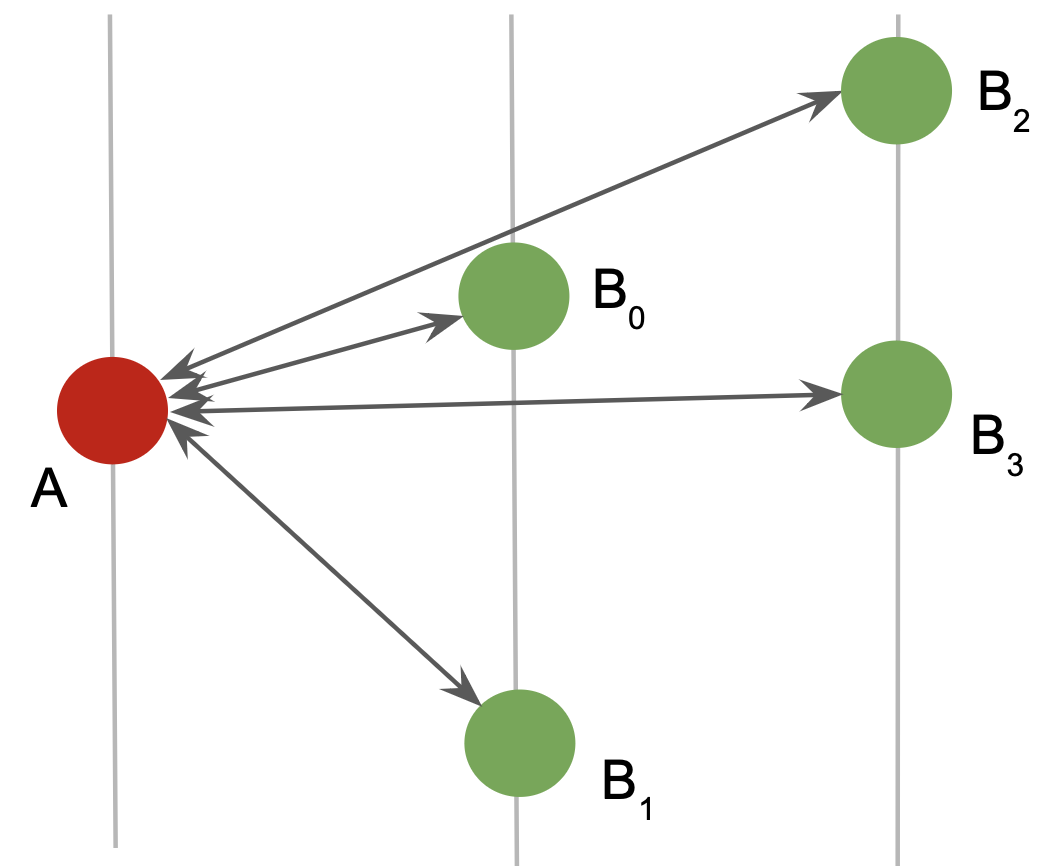
\includegraphics[width=0.42\linewidth]{images/5-gnn-algorithm/GMR-1.png}%
        \label{fig:GMR-1}%
        }%
    \hfill%
    \subfloat[]{%
        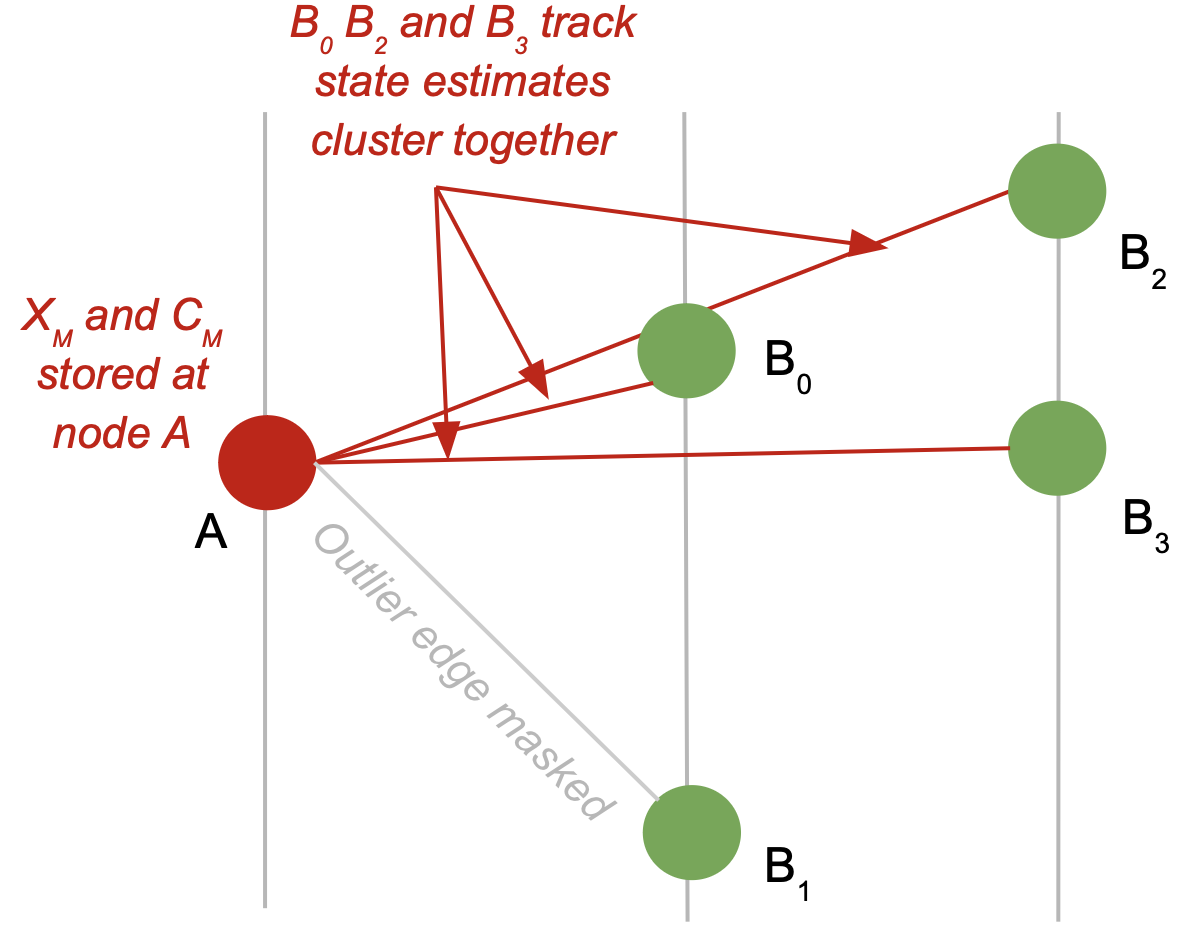
\includegraphics[width=0.57\linewidth]{images/5-gnn-algorithm/GMR-2.png}%
        \label{fig:GMR-2}%
        }%
    \caption{Illustration of GMR via clustering applied to graph networks. a) shows node $A$ and its local neighbourhood $B_j$ with bidirectional edge connections. b) shows the expected result of GMR applied to node $A$, where a merged track state $X_M$ is formed from states $X_{AB_0}$, $X_{AB_2}$, $X_{AB_3}$ clustered together and the corresponding merged state covariance $C_M$ formed from $C_{AB_0}$, $C_{AB_2}$, $C_{AB_3}$. An outlier connection has been identified, where the incoming $B_1 - A$ edge has been deactivated (dotted line) as any incoming state information from neighbour $B_1$ is deemed incompatible at node $A$.}
    \label{fig:GMR-example}
\end{figure}

The k-means clustering is implemented using the general case of $k=1$ to model the Gaussian mixture at each node as a single track with outlier connections. For the case where a node is located in close proximity to an intersection between two tracks, two or more clusters can be expected. In such a case, the mixture reduction process is declared impossible. This part of the network remains dormant until competing edges are deactivated and the mixture becomes more unimodal. 


\subsection{The Kullback-Leibler Divergence}
In order to establish whether clustering can occur for a given node, a distance measure is needed to serve as a threshold. The Kullback-Leibler (KL) divergence, $d_{KL}$, is a measure of the statistical distance between two Gaussian probability distributions \cite{KL, FRUHWIRTH19971}, and is used in the k-means algorithm to determine if track states can be grouped into a cluster. The $d_{KL}$ between track state estimates $X_{ij}$ and $X_{ik}$ is given by Eq \eqref{eqn:kullback-leibler}.

\begin{equation}
    d_{KL} = tr[(C_{ij} - C_{ik})(G_{ij} - G_{ik})] + (X_{ij} - X_{ik})^{T}(G_{ij} + G_{ik})(X_{ij} - X_{ik})
    \label{eqn:kullback-leibler}
\end{equation}

The optimal $d_{KL}$ threshold will differ for each node depending on its local neighbourhood. For example, consider a node with a high empirical variance of edge orientation in its neighbour connections, $\sigma_{e}$. The corresponding $d_{KL}$ threshold will be larger in comparison to a node with a small $\sigma_{e}$, where neighbour connections are more closely orientated. To determine the optimal $d_{KL}$ threshold between track state estimates $X_{ij}$ for a given node, a SVM classifier was trained against a MC simulation, using pairwise $d_{KL}$ and $\sigma_{e}$ as input features. See Section \ref{chapter-6-kl-threshold} for details on the implementation of the SVM classifier.





\section{Information Aggregation}

\subsection{Message Passing}
The message passing mechanism of graph networks is leveraged in order to improve the precision about track state parameters on a local and global scale. During the previous stage, reduced Gaussian mixtures were formed for nodes where clustering was successful. For a given node $i$, $X^M$ and $C^M$ are propagated to all neighbour nodes $j$ which have their edge connection $i \rightarrow j$ active. If clustering was unsuccessful for a particular node, this part of the network remains dormant until a merged state is received via message passing during later stages of the algorithm. Track state information can be propagated in both directions along active network edges. Bidirectional message passing ensures that the compatibility of propagated states can be validated and assessed against each node's local neighbourhood.


\subsection{Validation}
Once state information has been propagated to neighbours, the parameter estimation begins with a linear projection of the incoming track state onto the subspace of measurements. As illustrated in Figure \ref{fig:extrapolation}, for a given node $i$ each incoming $X^M$ is projected via a measurement matrix $H$, which relates the incoming track state to the measurement values. See Section \ref{gnn-application-toy-model} for implementation of matrix $H$. In order to validate if the connection between node $i$ and $j$ is compatible, the Mahalanobis distance, $\Delta \chi^{2}_{ij}$, is calculated using the residual between the projected state $HX$ and the measurement at the neighbour node. If $\Delta \chi^{2}_{ij} < d_{\chi}$, where $d_{\chi}$ is a tuned distance threshold, the connection is deemed compatible and the state can be extrapolated via a KF. If $\Delta \chi^{2}_{ij} > d_{\chi}$ then the connection is deemed incompatible and the corresponding edge is deactivated. The threshold $d_{\chi}$ represents the maximum $\Delta \chi^{2}_{ij}$ acceptable for an incoming track state.

\begin{figure}[htbp]
        \centering
        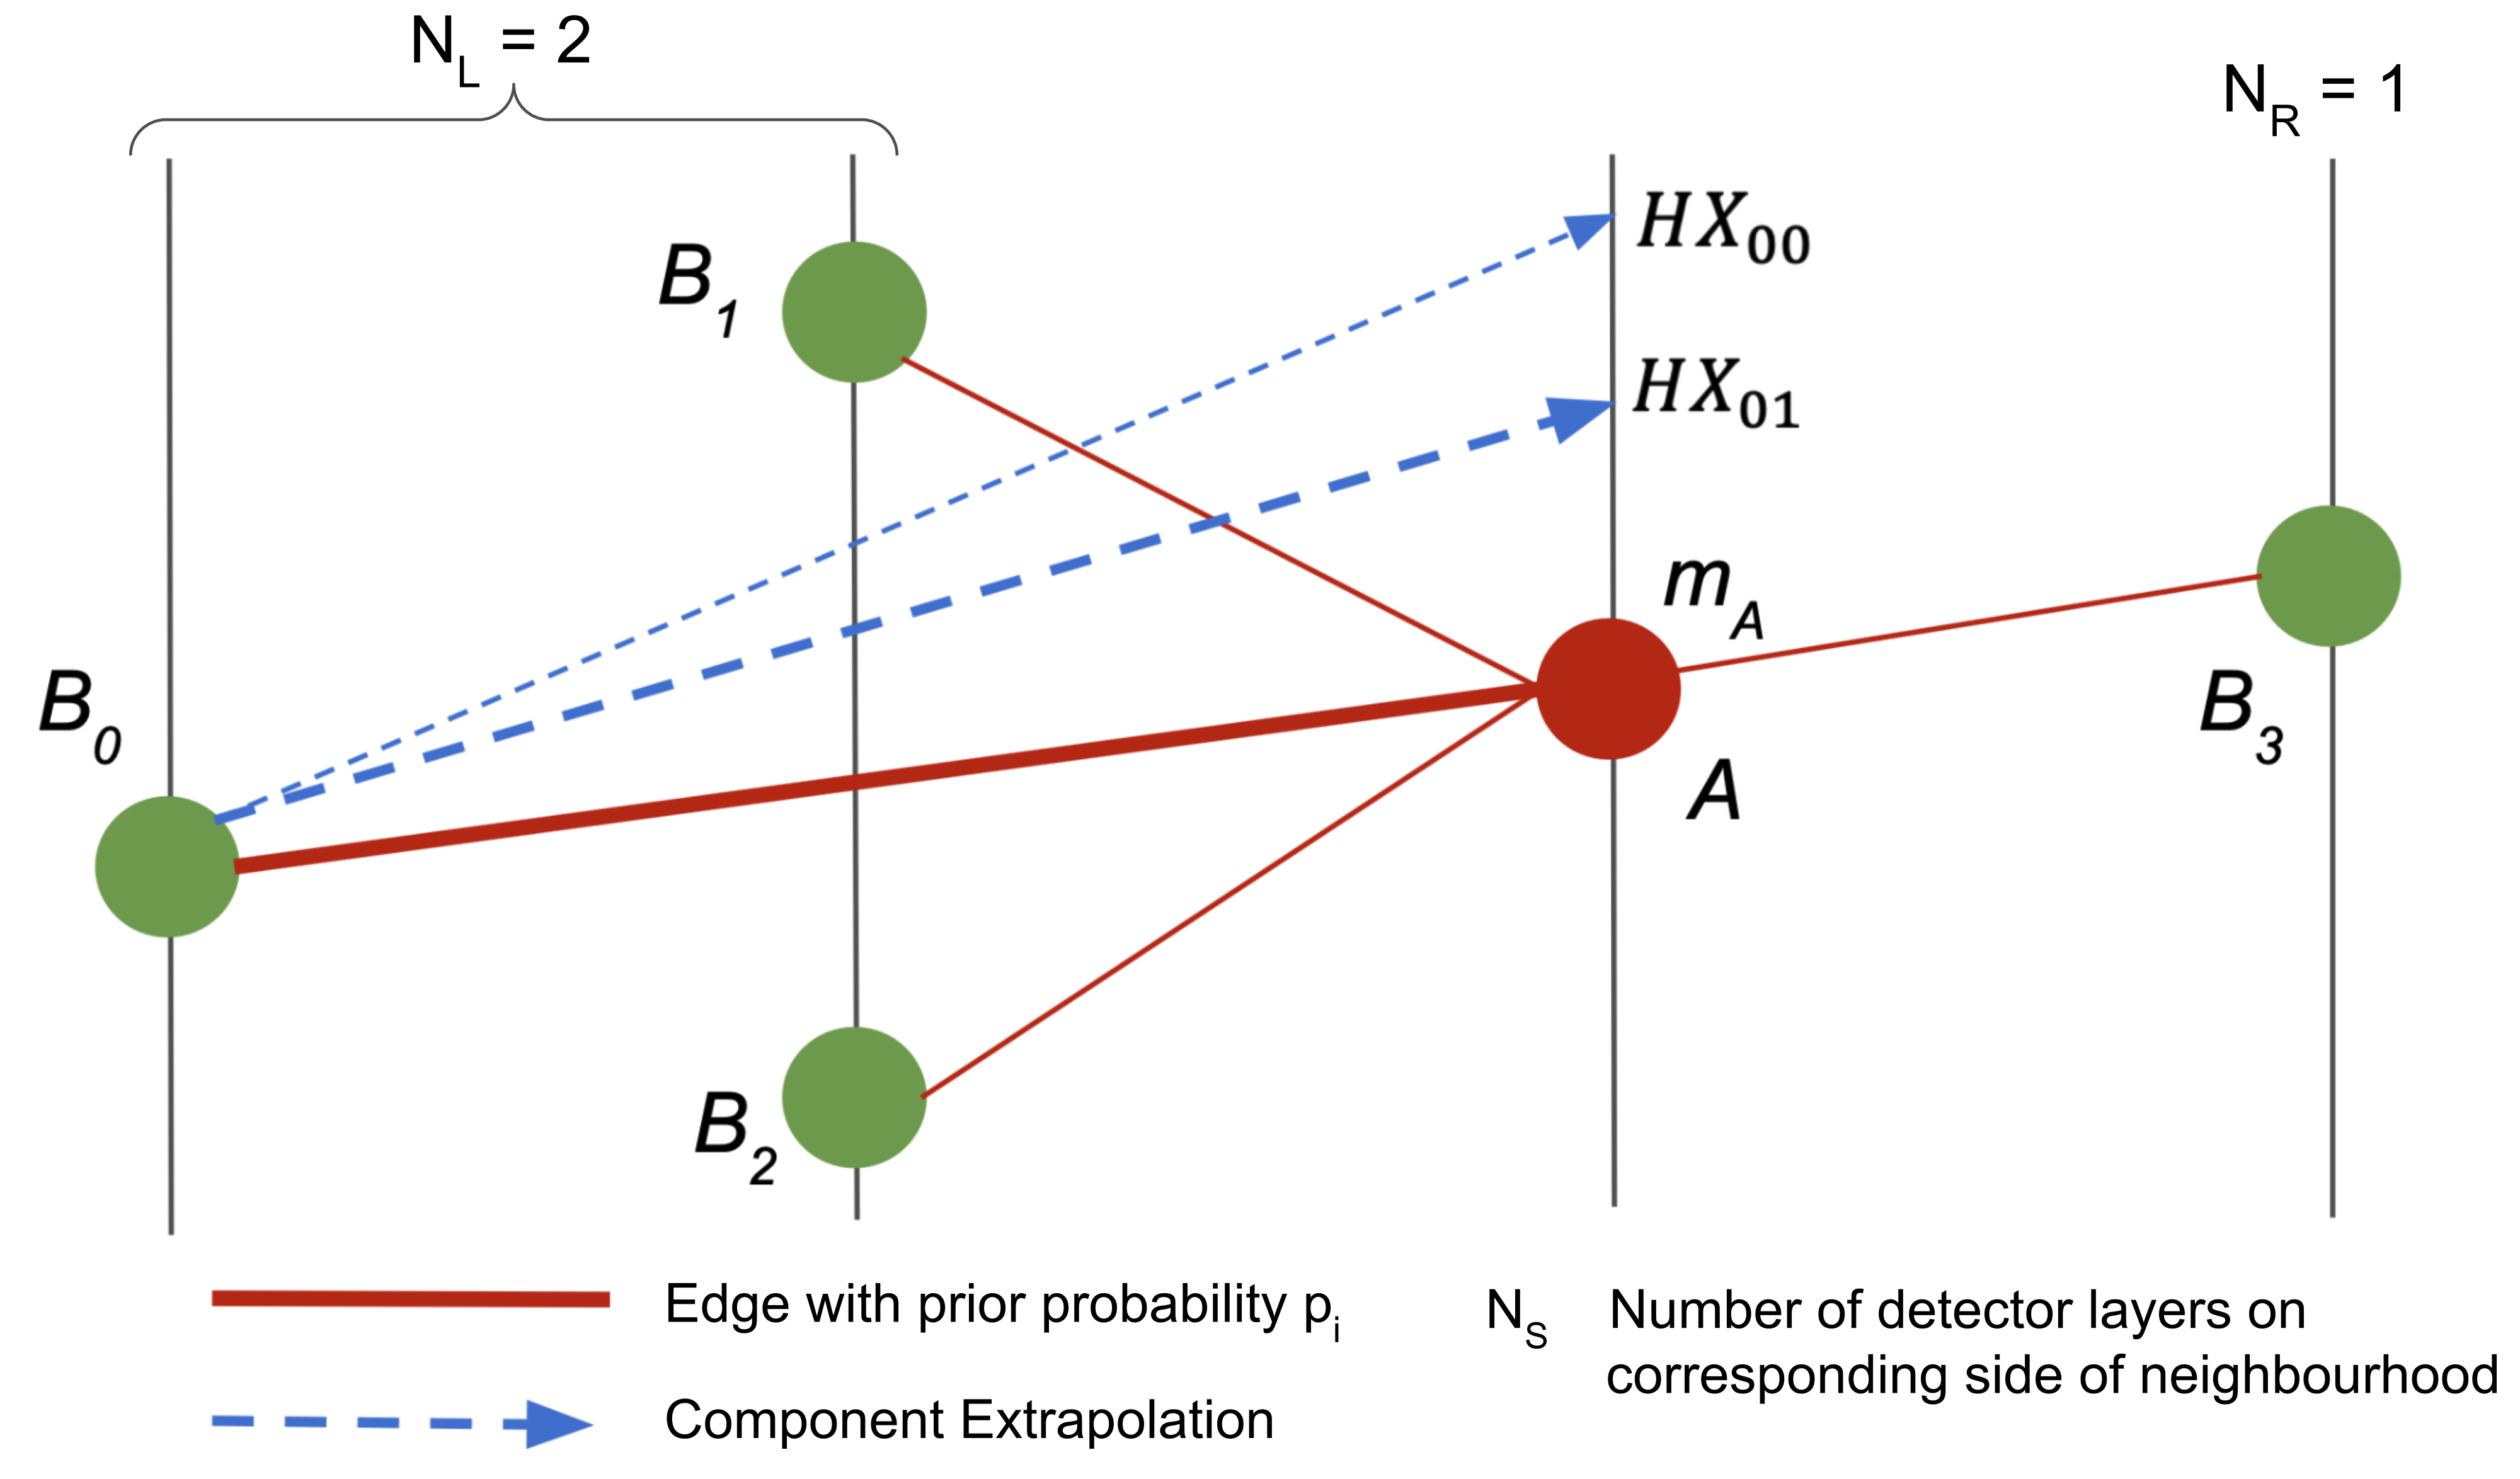
\includegraphics[width=0.87\textwidth]{images/5-gnn-algorithm/gnn-extrapolation.png}
        \caption{Illustration of track state estimates $X_{00}$ and $X_{01}$ being projected from node $B_0$ to node $A$ via a measurement matrix $H$ into the subspace of measurements. $m_A$ is the measurement at node $A$. The corresponding residual between $m_A$ and the projected incoming state from $B_0$ is used to compute the Mahalanobis distance $\Delta \chi^{2}$ to determine if the incoming state is compatible with $m_A$. $N_L$ indicates the number of detector layers on the left side of node $A$'s local neighbourhood, and $N_R$ indicates the number of detector layers on the right side.}
        \label{fig:extrapolation}%
\end{figure}


\subsection{KF Update and Extrapolation}
\label{chapter-5-kf-extrapolation}

For compatible incoming states where $\Delta \chi^{2}_{ij} < d_{\chi}$, the KF update is applied in order to compute the extrapolated track state estimate $\tilde{X}_{ij}$ and the corresponding extrapolated covariance matrix $\widetilde{C}_{ij}$. The KF is implemented via the Python library \textit{Filterpy} \cite{filterpy}. $\tilde{X}_{ij}$ and $\widetilde{C}_{ij}$ are given by Eqs. \eqref{eqn:extrapolation},

\begin{equation}
\tilde{X}_{ij} = F_{ij} X_{ij}^{M}, \qquad \tilde{C}_{ij} = F_{ij} \biggl( \sum C_{ij}^{M} + Q \biggl) F^{T}_{ij}
\label{eqn:extrapolation}
\end{equation}

where $F_{ij}$ is the state transition Jacobian from nodes $i$ to node $j$, and $Q$ is the process noise matrix. See Section \ref{gnn-application-toy-model} for implementation of the KF update, Jacobian $F$ and process noise $Q$. 






\section{Updating Network State}
\label{gnn-updating-network-state}

As the network evolves and specific connections are deactivated, the local track parameter estimates change at each node. Therefore, the corresponding edge weights $w_{ij}$ should reflect this for the strength of each connection, and hence $w_{ij}$ are updated. For the connection between nodes $i$ and $j$, the updated edge weights $\widetilde{w}_{ij}$ are computed using the normalised Gaussian measurement likelihood given by Eq. \eqref{eqn:likelihood}stated, where $S_{ij}$ is the joint measurement covariance matrix.

\begin{equation}
\beta_{ij} = (2 \pi \lvert S_{ij} \rvert )^{-1/2}  e^{-\Delta \chi^{2}_{ij} / 2}
\label{eqn:likelihood}
\end{equation}


The updated edge weights $\widetilde{w}_{ij}$ are given by Eq. \eqref{eqn:weights}. The denominator $\sum_{k}w_{ik}\beta_{ik}$ is the summation of the product of weights and likelihoods in the neighbourhood of a given node $i$. The updated weights $\widetilde{w}_{ij}$ are also divided by the number of detector layers on either side of its neighbourhood $N_S$, in order to account for the probability that a track passing through node $i$ was detected at layer $L$. For a given node, if $\widetilde{w}_{ij} < 0.1$, the corresponding edge connection is automatically deactivated as the likelihood of compatibility of this incoming track state is extremely low. This forms part of the mechanism for edge activation and deactivation.

\begin{equation}
\widetilde{w}_{ij} = \frac{1}{N_S} \frac{w_{ij}\beta_{ij} p_{ij}}{\sum_{k}w_{ik}\beta_{ik}}
\label{eqn:weights}
\end{equation}

$g_i(X)$ at each node is then composed of updated components, given by Eq \eqref{eqn:updated-gaussian-mixture}.

\begin{equation}
g_i(X) = \sum_{j} \widetilde{w}_{ij}\phi_{ij}(X, \widetilde{X}_{ij}, \widetilde{C}_{ij})
\label{eqn:updated-gaussian-mixture}
\end{equation}

Following this update, the algorithm iterations repeat. A further GMR would follow, clustering on updated track state estimates. This allows further ambiguities to be resolved and precision of track states to be increased at each additional stage.






\section{Graph Splitting and Track Extraction}
\label{gnn-track-extration}

The GNN-based framework is designed such that it is possible to iteratively discover track candidates after each stage. As shown in Figure \ref{fig:flowchart}, a track extraction algorithm is executed after the GMR and Information Aggregation stages.

Initially, the graph network is split into smaller components, taking into account only edges which remain active. A CCA is applied to the graph network by using the NetworkX built-in function \textit{weakly connected components}. This ensures that smaller, more manageable subgraphs can be separated from the main network.

The criteria that a subgraph must possess in order to be considered for track extraction is as follows. Subgraphs must contain a minimum number of four nodes within the volume of interest. There must exist only one node per layer, such that there are no are intersecting tracks or holes within the track candidate. 

If the above criteria are met, a KF is then applied in order to perform a track fit. As opposed to applying the KF on one track segment between two nodes, similar to the method used in Section \ref{chapter-5-kf-extrapolation} for state extrapolation, the KF for track fitting must consider the whole chain of track segments. Here, the filter iteratively predicts and updates track state parameters as it receives $X_{ij}$ and $C_{ij}$ from each subsequent node in the subgraph.

In order to assess the quality of the track fit the p-value is computed from the $\chi^2$ statistic. The p-value obtained must be greater than 0.01. Such subgraphs that fulfill all conditions are defined as good track candidates and extracted from the network, where their corresponding nodes and edges are removed. Any subgraphs that do not meet the above criteria for track extraction, remain in the graph network for further processing.





\section{Application on a Simple Model}
\label{gnn-application-toy-model}

Mention here that only a linear model was used in this instance, where the track state estimate comprised of a 2x1 vector, with measurement y and inverse track inclination tau. The extrapolation and hence KR update that was used here was therefore linear too and 2x2 - will have to show a different transition Jacobian matrix.

% This indicates, that $\sigma_{e}$ is also an important feature in used as a discriminating feature when clustering. 

% TODO: mention here that the linear track state model was used and reference the section

% The excitation and inhibition rules of individual GNN nodes will be designed to facilitate the “simple-to-complex” approach for “hits-to-tracks” association, such that the network starts with relatively “easy” areas of an event (low hit density) and gradually progresses towards more complex areas (high hit density). 

% \begin{itemize}
% \item Application on a simple toy mc model and heat network - track extracted and metrics
% \end{itemize}

A 2-dimensional simulation with seven tracks, each with ten hits, was created, see Figure \ref{fig:ground-truth}. The graph network was formed using a many-to-one mapping of hits-to-nodes, where close proximity hits were merged into one node. The threshold for close proximity hits was determined by considering the distance distribution between hits located in the same layer. In order to build edge connections in the graph network and reduce all possible combinatorics between node pairs, an edge-predictor method was devised. The predictor uses a simple calculation whereby the track inclination of neighbouring nodes is calculated. If the inclination of a neighbour spanning up to two layers apart is within a particular range, then this edge is compatible and a connection is established between the nodes. The network is initialised with its corresponding track state estimates $X_{ij}$, covariance matrices $C_{ij}$ and MC truth particle.

In order to efficiently resolve ambiguities, a method was devised to automatically determine a suitable region for initiating the pattern recognition. For a given node, the variance of edge orientation $\sigma_e^2$ of its neighbourhood was considered. Figure \ref{fig:heat-map} shows a heat map, indicating ``hot'' nodes (white) which represent nodes with a high degree (number of edges associated to the node), whereas ``cold'' nodes (orange - red) indicate regions with fewer ambiguities to resolve. This indicates that the node degree is an indirect characteristic of how complex a local neighbourhood is and provides a method to determine where pattern recognition should begin on a graph network in order to resolve incompatible edge connections. Nodes with $\sigma_e^2 > 0.8$ were temporarily removed and the pattern recognition was initially applied to the remaining network.

Each pairwise connection between two nodes forms a track state estimate $X_{ij}$ given by Eq. \eqref{eqn:track-state-estimate}. $X_{ij}$ comprises of the measurement at node $i$, $m_i$ and the track inclination to the neighbouring node $j$, given by $t_{ij} = (m_i - m_j) / (x_i - x_j)$, modelling the segment as a straight line. The joint measurement covariance matrix, $S$, for connections $i \rightarrow j$ are stated in Eq. \eqref{eqn:track-state-estimate}, where $\sigma_0^{2}$ is the error due to measurement in the $xy$ plane initialised to 100$\mu m$. Additionally, negligible error is assumed in the x measurement due to the low thickness of Pixel sensors. Matrix $G$ relates the measurements to the state vector $X_{ij}$ using a linear extrapolation where $dx = x_i - x_j$. The state covariance $C_{ij}$ is derived using the standard linear algebra approach, where $C_{ij} = GSG^T$. 

\begin{equation}
X_{ij} = \begin{bmatrix} m_i \\ t_{ij} \end{bmatrix} \quad S = \begin{bmatrix} \sigma_0^{2} & 0 \\ 0 & \sigma_0^{2} \end{bmatrix}  \quad G = \begin{bmatrix} 1 & 0 \\ 1/dx & -1/dx  \end{bmatrix}
\label{eqn:track-state-estimate}
\end{equation}

Figure \ref{fig:example-application-1} shows an example of the GNN-based algorithm described in Section \ref{development} applied to this simulated network. Figure \ref{fig:weakly-connected-graphs} displays the simulated network where nodes with $\sigma_e^2 > 0.8$ have been removed and a CCA has been applied, reducing the computational complexity in further stages as three smaller subgraphs have been identified. The extracted track candidates are shown in Figure \ref{fig:extracted-candidates-1}. Outlier edge connections have been successfully removed, as this particular simulation shows successful extraction of all seven truth tracks within two stages.

Figure \ref{fig:example-application-2} shows another simulation of a simple track model with application of the GNN algorithm. Similarly, nodes with $\sigma_e^2 > 0.8$ have been removed and a CCA has been applied. Figure \ref{fig:intermediate-step} indicates the results of the network state after the GMR stage, where outlier edge connections have been identified and are represented in grey. A precision of 65\% was achieved on identifying correct outlier connections with respect to MC truth. A fast convergence was achieved in extracting 6/7 candidates after the first stage and the remaining subgraphs are propagated to further stages. 


\begin{center}
\begin{figure}[htbp]%
    \centering
    \subfloat[\centering Simulation of seven truth tracks]{{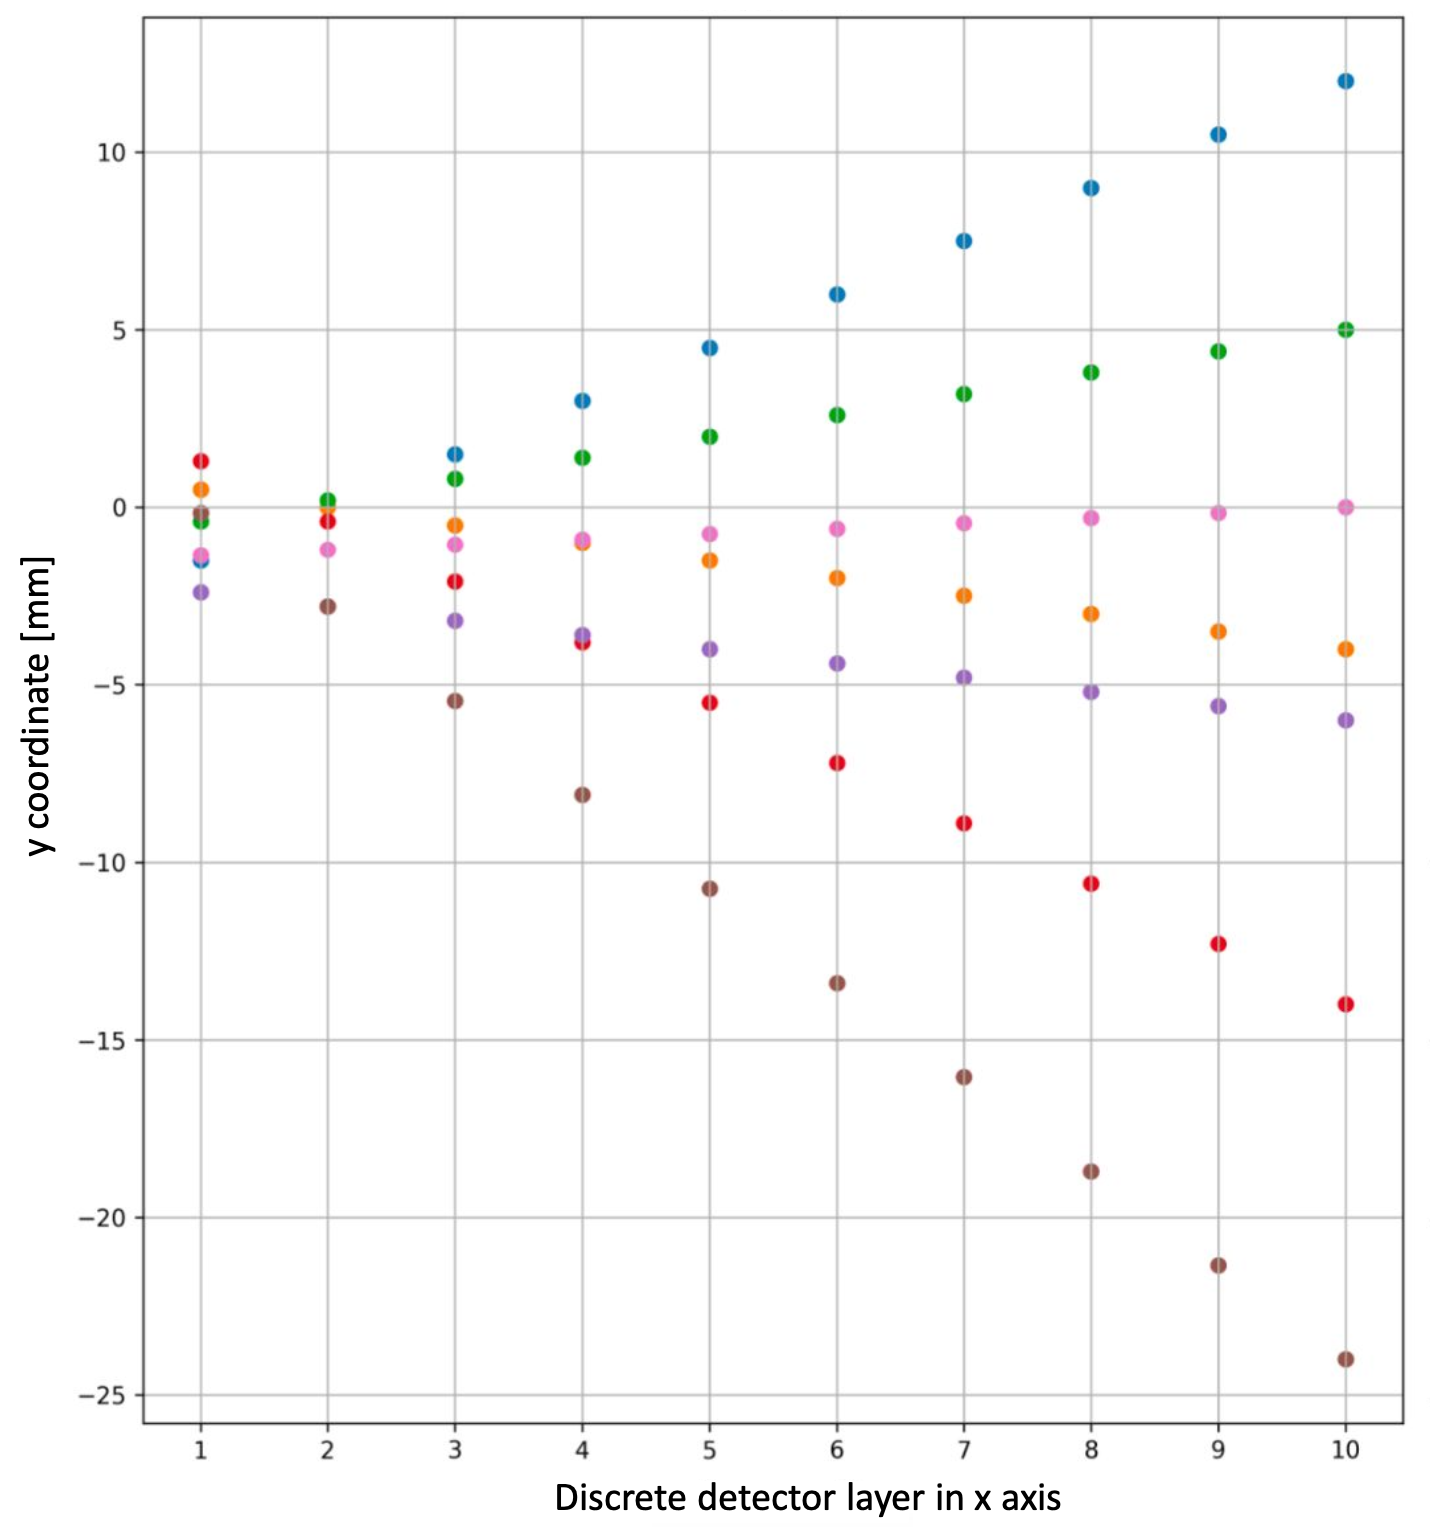
\includegraphics[width=8cm]{images/5-gnn-algorithm/ground-truth.png} } \label{fig:ground-truth}}%
    \hfill
    %\qquad
    \subfloat[\centering Graph network plotted as a node-degree heat map]{{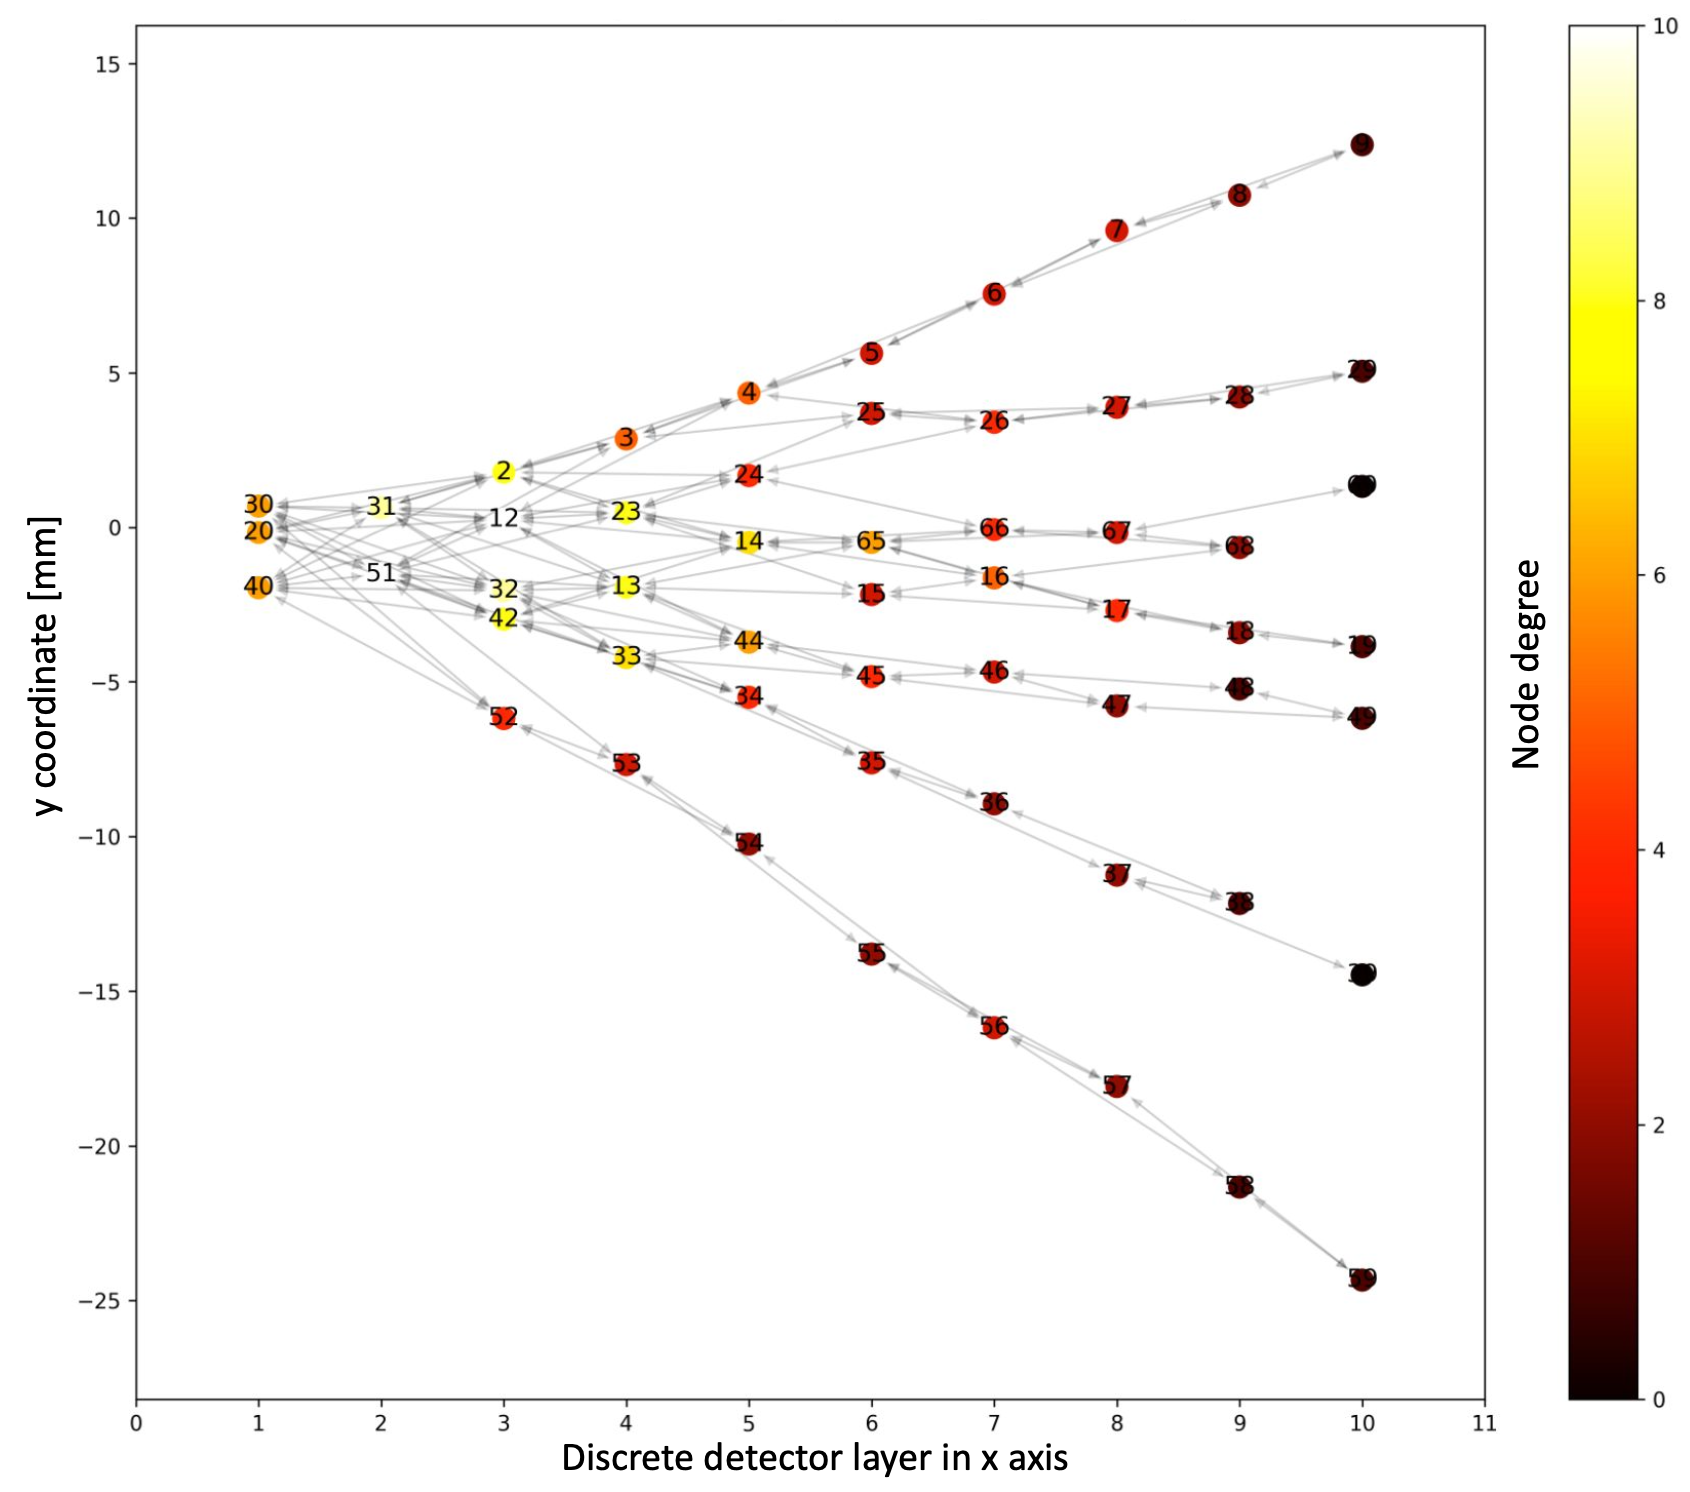
\includegraphics[width=11cm]{images/5-gnn-algorithm/heatmap-network.png} } \label{fig:heat-map}}%
    \caption{a) Simple 2-dimensional simulation of seven truth tracks where each track contains ten hits; one hit per layer. Each colour represents a different track. b)  Conversion of the simulated hits in a), to a graph network containing nodes and edges. Close proximity hits are merged into the same node where necessary and predicted edge connections are formed using a pair predictor. The heat map represents node degree, where ``hot'' nodes (white) contain many edge connections, whereas ``cold'' nodes (orange - red) contain fewer edge connections.}%
    \label{fig:setup}%
\end{figure}
\end{center}


\begin{center}
\begin{figure}[htbp]%
    \centering
    \subfloat[\centering Weakly connected graph networks]{{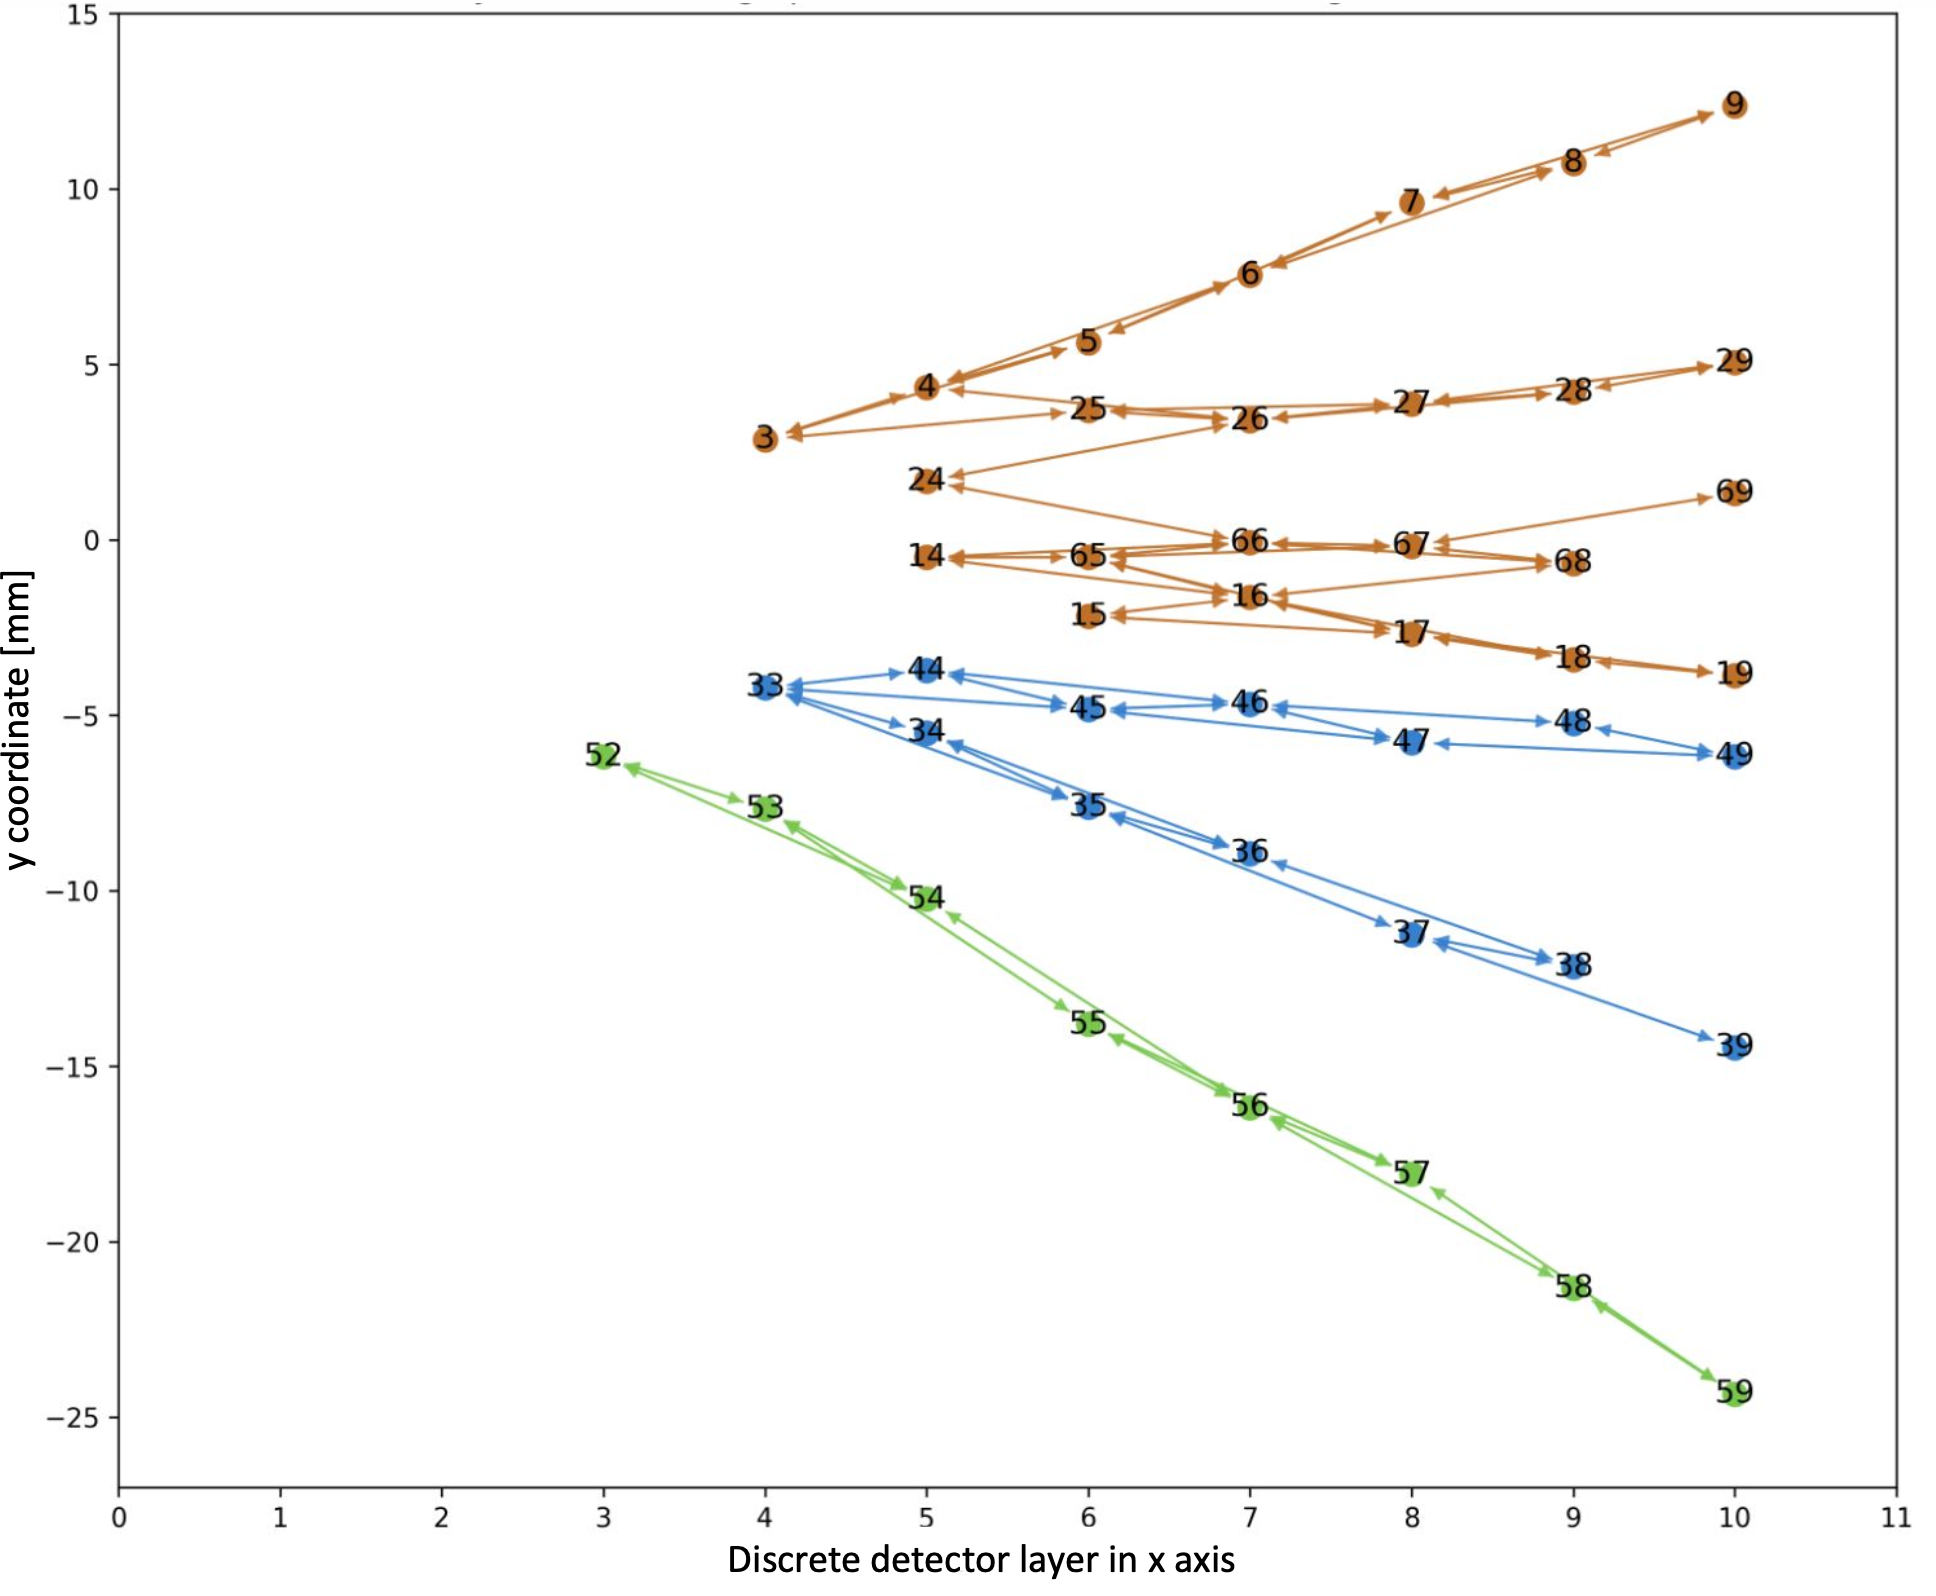
\includegraphics[width=11cm]{images/5-gnn-algorithm/mc-example-1.png} } \label{fig:mc-example-1}}%
    \hfill
    %\qquad
    \subfloat[\centering Extracted track candidates]{{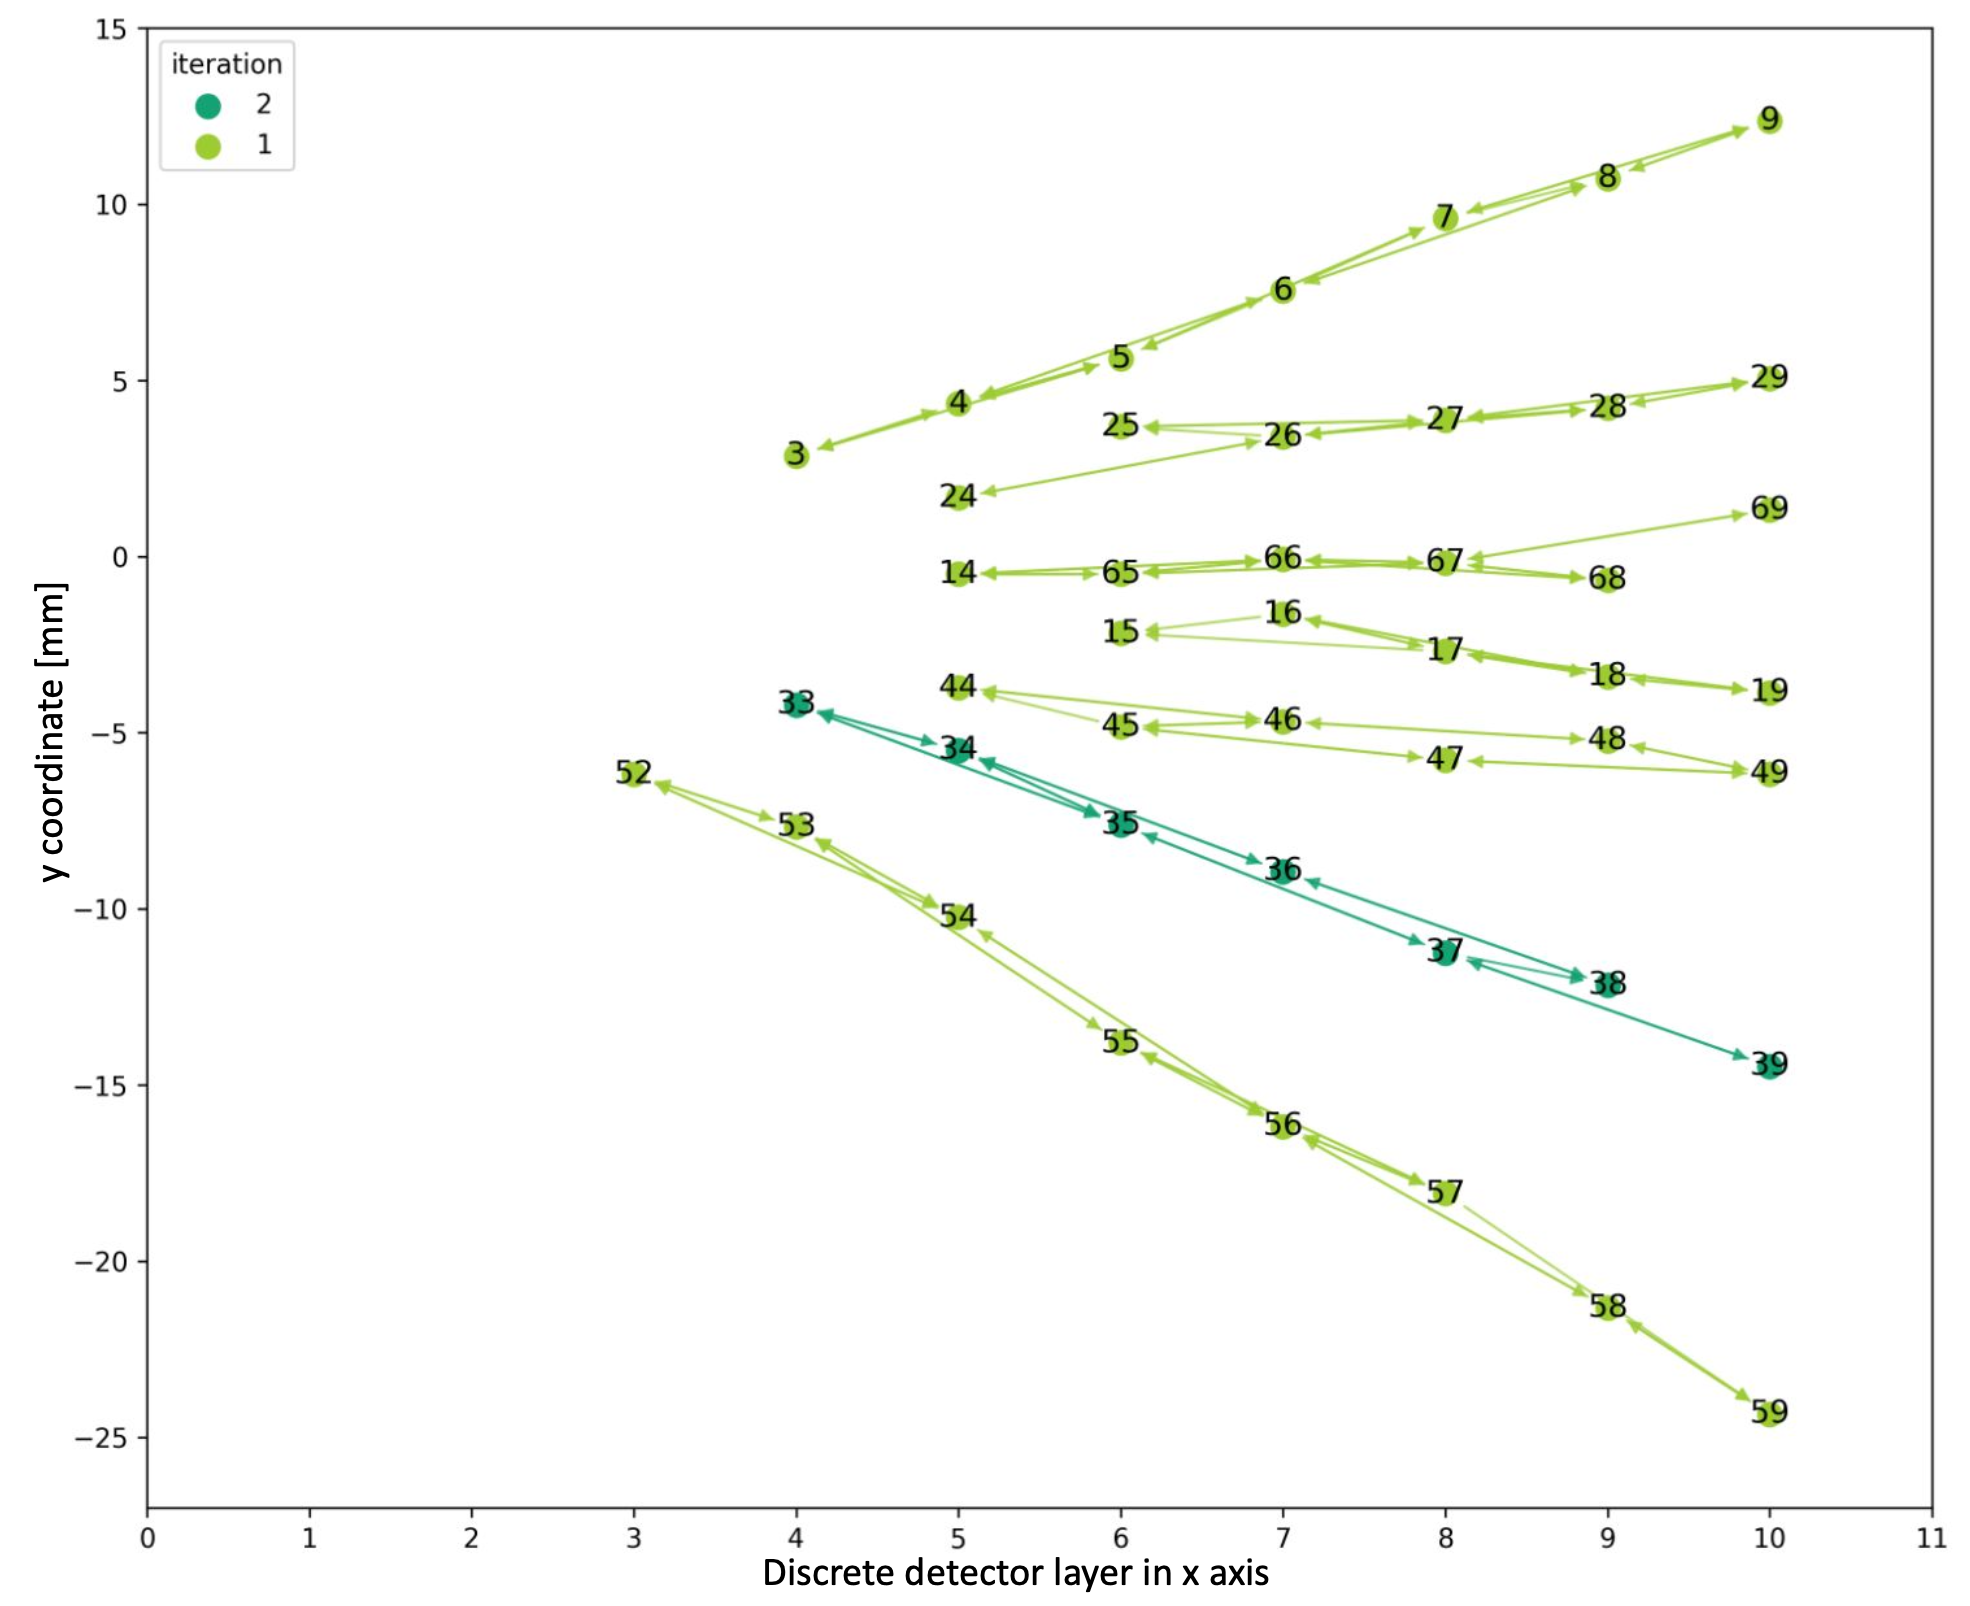
\includegraphics[width=11cm]{images/5-gnn-algorithm/mc-example-2.png} } \label{fig:mc-example-2}}%
    \caption{Results of the GNN-based algorithm for track finding a) Simulated graph network where nodes $\sigma_e^2 > 0.8$ are removed and CCA is applied. Each colour represents a separate network. b) The extracted track candidates after GMR and Information Aggregation.}%
    \label{fig:example-application-1}%
\end{figure}
\end{center}




%\section{Conclusions}
